% Chapter Template

\chapter{Introduction} % Main chapter title

\label{Chapter1}

\lhead{Chapter 1. \emph{Introduction}} % Change X to a consecutive number; this is for the header on each page - perhaps a shortened title
\lipsum[1]\\
\lipsum[1]\\
\lipsum[1]

Figure~\ref{fig:ovexamples} below represents each of the situations given in the previous examples, for different values of $J$. Given 4 functions (a), the black functions in (b), (c) and (d), represent the Order-Value functions for the Min-min, Min-max and VaR-like problems, respectively. 
\begin{figure}[H]
     \centering
     \begin{subfigure}{0.32\textwidth}
         \centering
         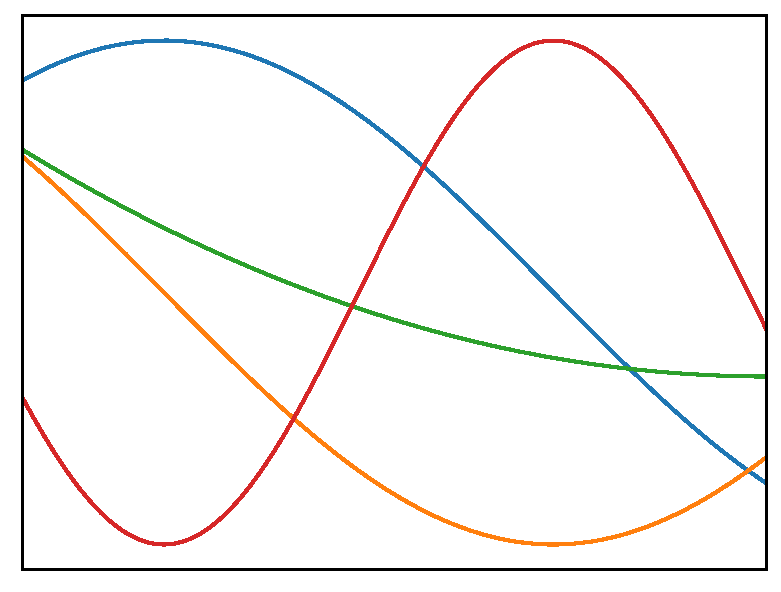
\includegraphics[width=\textwidth]{pictures/scenarios.pdf}
         \caption{$m=4$}
         \label{fig:scenarios}
     \end{subfigure}
     \hfill
     \begin{subfigure}{0.32\textwidth}
         \centering
         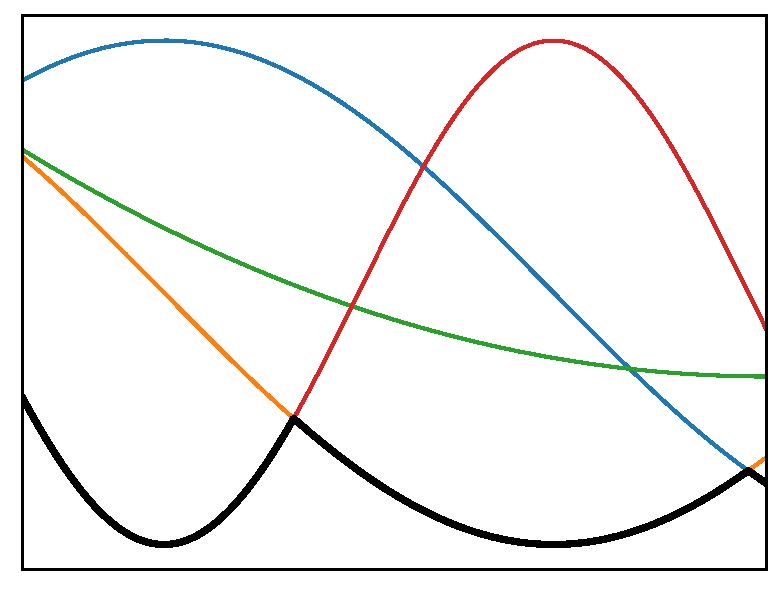
\includegraphics[width=\textwidth]{pictures/minimin.pdf}
         \caption{$J=\{1\}$}
         \label{fig:minimin}
     \end{subfigure}
     \hfill
     \begin{subfigure}{0.32\textwidth}
         \centering
         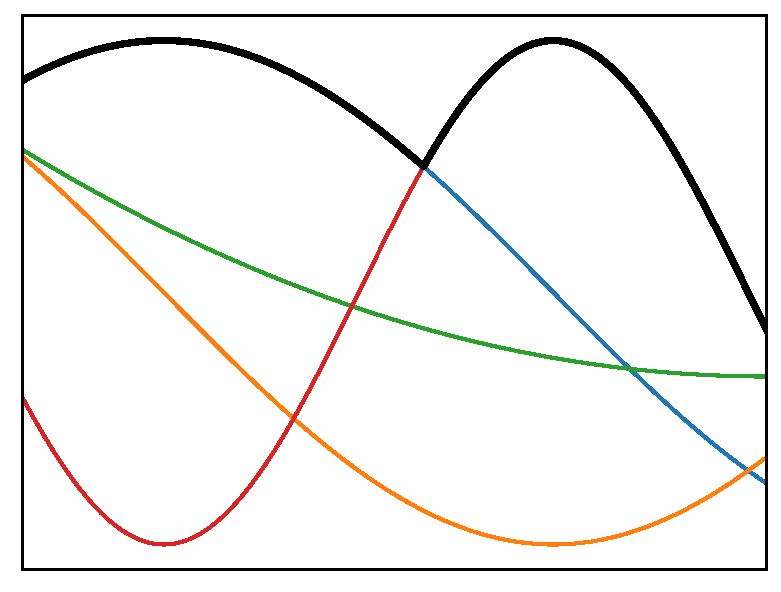
\includegraphics[width=\textwidth]{pictures/minimax.pdf}
         \caption{$J=\{4\}$}
         \label{fig:minimax}
     \end{subfigure}

     \begin{subfigure}{0.32\textwidth}
         \centering
         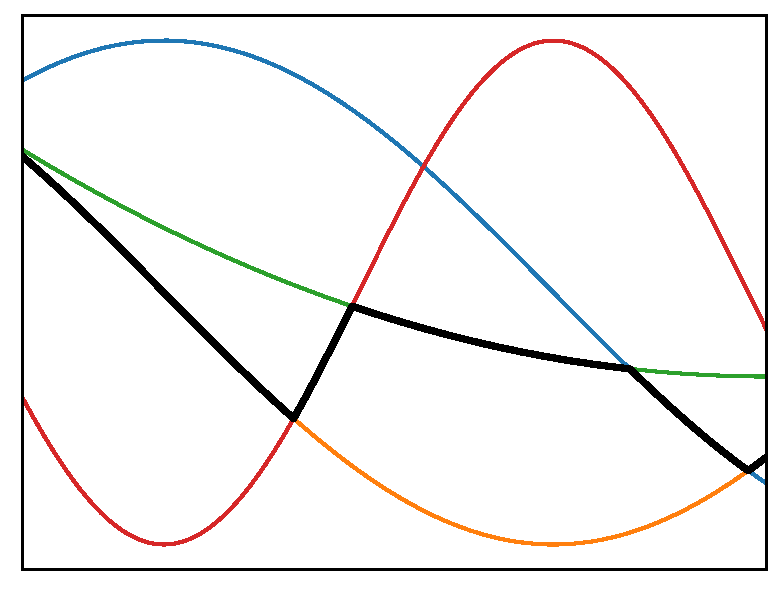
\includegraphics[width=\textwidth]{pictures/var.pdf}
         \caption{$J=\{2\}$}
         \label{fig:var}
     \end{subfigure}
     \hfill
     \begin{subfigure}{0.32\textwidth}
         \centering
         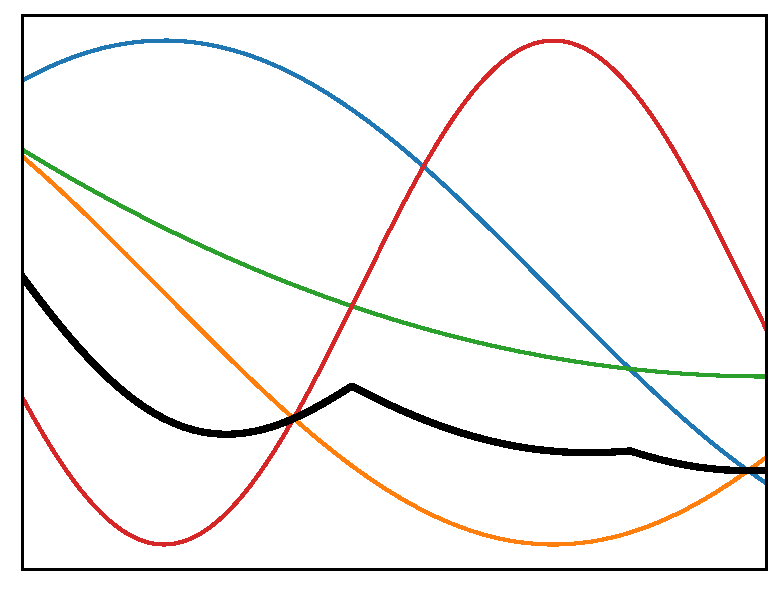
\includegraphics[width=\textwidth]{pictures/lovo.pdf}
         \caption{$J=\{1,2\}$}
         \label{fig:lovo}
     \end{subfigure}
     \hfill
     \begin{subfigure}{0.32\textwidth}
         \centering
         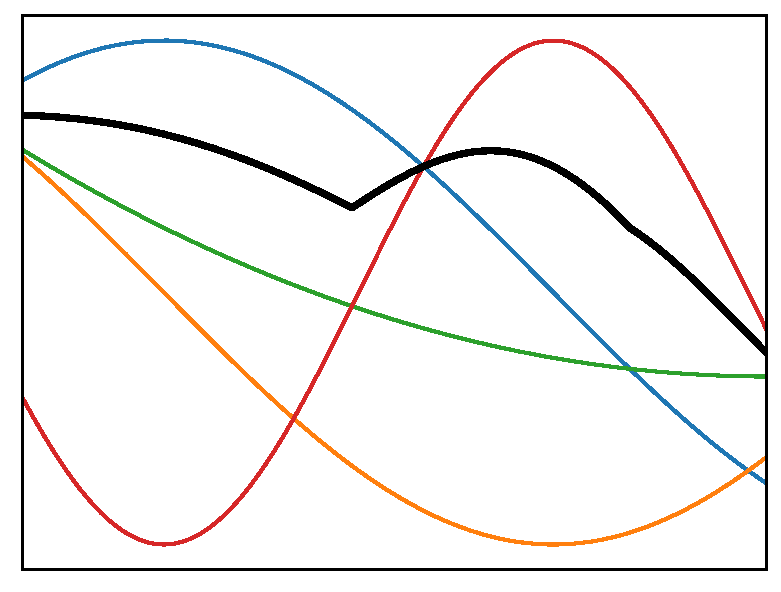
\includegraphics[width=\textwidth]{pictures/cvar.pdf}
         \caption{$J=\{3,4\}$}
         \label{fig:cvar}
     \end{subfigure}
        \caption{Order-Value functions for $J\subset\{1,2,3,4\}$.}
        \label{fig:ovexamples}
\end{figure}

